\documentclass{article}
\usepackage{amsmath, amssymb, mdwlist, graphicx, hyperref}
\usepackage{listings,color}
\usepackage{wrapfig}
\usepackage[usenames,dvipsnames]{xcolor}
\definecolor{gray}{rgb}{0.97,0.97,0.97}
\lstset{%
language=C,%
%backgroundcolor=\color{gray},
emph={putpixel},
emphstyle=\bf,
tabsize=4,
framesep=5pt,
mathescape=true,
xleftmargin=0.1cm,
xrightmargin=0.1cm,
frame=lines,
%basicstyle=\ttfamily,
%keywordstyle=\color{Blue},
%commentstyle=\color{OliveGreen},
%stringstyle=\color{MidnightBlue},
columns=flexible,
%showstringspaces=false
}

\newcommand{\mpar}[1]{\marginpar{\textit{#1}}}
\newcommand{\norm}[1]{\Vert #1 \Vert}
\DeclareMathOperator{\argmax}{argmax}
\DeclareMathOperator{\argmin}{argmin}
\newenvironment{solution}{\paragraph{Solution.}$\,$ }{\vskip 3mm\hrule}
\newenvironment{exercise}[2]{\paragraph{Exercise #1 (#2pt).} }{
\medskip}
\newcommand{\bbR}{\mathbb{R}}
\newcommand{\bw}{\mathbf{w}}
\newcommand{\bx}{\mathbf{x}}
\newcommand{\bd}{\mathbf{d}}
\newcommand{\bb}{\mathbf{b}}
\newcommand{\by}{\mathbf{y}}
\newcommand{\bzero}{\mathbf{0}}
\newcommand{\bz}{\mathbf{z}}
\newcommand{\bSigma}{\mathbf{\Sigma}}
\newcommand{\bp}{\mathbf{p}}
\newcommand{\bP}{\mathbf{P}}
\newcommand{\bm}{\mathbf{m}}
\newcommand{\bc}{\mathbf{c}}
\newcommand{\bM}{\mathbf{M}}
\newcommand{\bV}{\mathbf{V}}
\newcommand{\bK}{\mathbf{K}}
\newcommand{\bD}{\mathbf{D}}
\newcommand{\bA}{\mathbf{A}}
\newcommand{\bX}{\mathbf{X}}
\newcommand{\bY}{\mathbf{Y}}
\newcommand{\bR}{\mathbf{R}}
\newcommand{\bI}{\mathbf{I}}
\newcommand{\bS}{\mathbf{S}}
\newcommand{\bT}{\mathbf{T}}
\newcommand{\balpha}{\boldsymbol{\alpha}}
\newcommand{\pt}[2]{\left(\begin{array}{c}#1\\#2\end{array}\right)}

\begin{document}
\title{MTAT.03.015 Computer Graphics (Fall 2013)\\
Exercise session VII: Lighting}
\author{Konstantin Tretyakov, Ilya Kuzovkin}
\date{October 21, 2013}
\maketitle

Today we shall study the basics of OpenGL lighting, and the use of fragment shaders. As usual, the base code is provided in the \texttt{practice07.zip} archive on the course website or via the course github page. Download, unpack and open it. You will need to submit your solution as a zipped archive file.

\section{OpenGL pre-3.x Lighting}
As you should remember from the lecture, OpenGL versions prior to 3.1 provide a bunch of convenient functions to implement the \emph{per-vertex Phong lighting} model.
%\footnote{In the later versions those functions are separated into what is called a \emph{compatibility context}, \url{http://www.opengl.org/wiki/Core_And_Compatibility_in_Contexts}.}
To use it you have to do the following:
\begin{enumerate}
\item Turn on lighting computations using \verb#glEnable(GL_LIGHTING)#, and one or more light sources using \verb#glEnable(GL_LIGHT#$x$\verb#)#,
\item Configure position/direction for each light source using\\ \verb#glLightfv(GL_LIGHT#$x$\verb#, GL_POSITION, ...)#. Note that it is important what coordinate frame this command is executed in, as the provided coordinates are transformed using the model-view matrix.
\item Configure \emph{ambient}, \emph{diffuse} and \emph{specular} light emission parameters of the Phong model for each light source using\\
\verb#glLightfv(GL_LIGHT#$x$\verb#, GL_AMBIENT, ...)#, etc.
For the ambient light it usually more reasonale to specify just a single overall \emph{ambient} term via \\
\verb#glLightModelfv(GL_LIGHT_MODEL_AMBIENT, ambient_light)# rather than provide it separately for each light source (which is possible, but makes less sense).
\item Configure \emph{ambient}, \emph{diffuse} and \emph{specular} light diffusion parameters for each surface using either the \verb#glMaterial# command or the combination of \verb#glEnable(GL_COLOR_MATERIAL)#, \verb#glColorMaterial# and \verb#glColor#.
\end{enumerate}
\begin{exercise}{1}{1}
Open the project \verb#1_Lighting#. The project renders three objects (the ``ground'', a ``blue sphere'' and a ``flying cube''). Your goal is to add lighting to the scene as described below.

\begin{enumerate}
\item First enable lighting computations using \verb#glEnable#. Once this is done, the scene will become dark. The \verb#glColor# commands that were used to specify pixel color before play no role any more.
\item Now start adding lights one by one. First enable the ambient light using \verb#glLightModel(GL_LIGHT_MODEL_AMBIENT ..)#. Let the ambient light intensity be $(0.1, 0.1, 0.1)$.
\item To have objects react to this light, you need to specify material parameters for them. You can usually do it by using the \verb#glMaterial# function, or by enabling \verb#GL_COLOR_MATERIAL#, and using \verb#glColorMaterial# together with \verb#glColor#. In this particular exercise you are requested to \emph{not} use \verb#GL_COLOR_MATERIAL#. Please, specify all material parameters using \verb#glMaterial#. This will allow you to continue to the next exercise later on.
\item Specify the following material properties:
\begin{enumerate}
\item \textbf{Ground}. Specular $(0, 0, 0)$, Ambient \& Diffuse: $(0.1, 1.0, 0.1)$.
\item \textbf{Cube}. Specular $(0, 0, 0)$, Ambient \& Diffuse: $(1, 0, 0)$.
\item \textbf{Sphere}. Specular $(1, 1, 1)$, Ambient \& Diffuse: $(0, 0, 1)$. Specular exponent (\verb#GL_SHININESS#) $20$.
\end{enumerate}
\item Now let us start adding actual light sources. First add the ``sun''. It will be a directional light source shining straight from above the ground with diffuse/specular intensity equal to $(0.4, 0.4, 0.4)$.
\item Next, add a positional light source, located exactly at the position of the flying cube. Let the diffuse \& specular intensity be $(0.5, 0.1, 0.1)$. Configure attenuation for this light source to be $\frac{1}{0.1 d^2}$. (Hint: see \verb#GL_CONSTANT_ATTENUATION#, \verb#GL_LINEAR_ATTENUATION#, \verb#GL_QUADRATIC_ATTENUATION#).
\item Finally, add a spotlight shining from the camera position straight forward. Set the diffuse \& specular intensity to $(1.0, 1.0, 1.0)$. Set the spotlight cutoff angle (\verb#GL_SPOT_CUTOFF#) to $20$ degrees, and the spotlight fall-off exponent (\verb#GL_SPOT_EXPONENT#) to $30$.
\end{enumerate}

\end{exercise}
In the end you should obtain an image like the one below.
\begin{center}
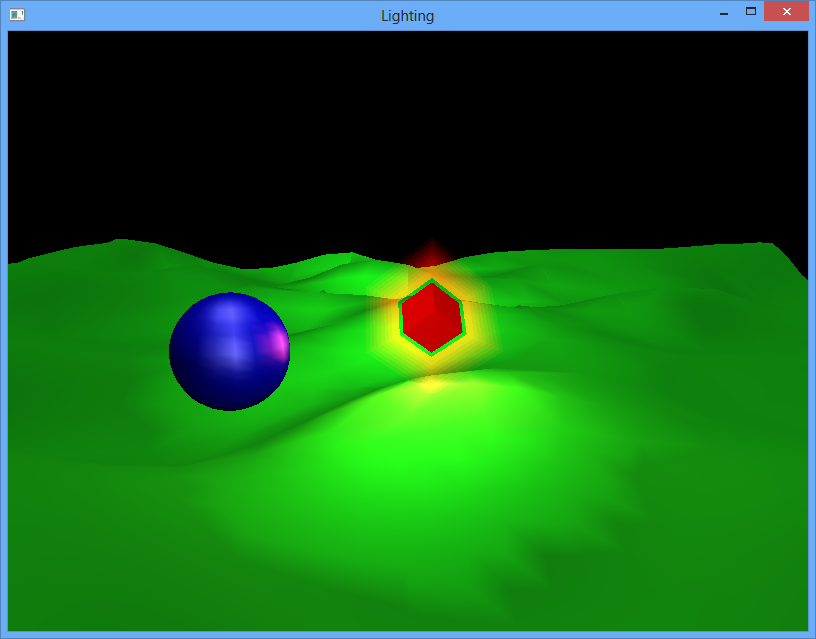
\includegraphics[width=1.0\textwidth]{lighting.png}
\end{center}

Note that OpenGL does not do gamma correction in its lighting computations. Some graphics cards, however, can perform on-the-fly sRGB-gamma-encoding as pixels are written to the framebuffer. To switch it on, use \verb#GLUT_SRGB# in your \verb#glutInitDisplayMode# call and do a \verb#glEnable(GL_FRAMEBUFFER_SRGB)#. See whether it makes any difference\footnote{E.g. my laptop does not react to \texttt{glEnable(GL\textunderscore FRAMEBUFFER\textunderscore SRGB)}.}


\section{GLSL, Per-vertex and Per-fragment Lighting}
Now let us try implementing the whole lighting logic manually in the shader program. We shall continue working with the \verb#1_Lighting# project.

\begin{exercise}{2}{1}
Uncomment the line 
\begin{lstlisting}
     per_vertex_lighting.use();
\end{lstlisting}
which is located somewhere near the end of the \texttt{main} function. Once you do it, the built-in OpenGL lighting computations will be disabled in favor of the shader programs \verb#lighting1_vertex.glsl# and \verb#lighting1_fragment.glsl#. Your task is to implement the lighting computations in the shader manually, so that the result would exactly match the \verb#GL_LIGHTING# solution you configured in the previous exercise using OpenGL's (now deprecated) fixed pipeline.

\noindent
You should keep the fragment shader intact. The vertex shader shows the implementation of the spotlight to get you started.
\end{exercise}

\begin{exercise}{3}{0.5}
So far we did \emph{per-vertex shading}, i.e. performing lighting computations for each vertex and interpolating the resulting colors. The result looks nice, but you can clearly see some ugly artifacts, in particular in how grainy the ``ground'' is lit. Let us now do per-fragment shading.

\noindent
Comment out the line \verb#per_vertex_lighting.use();# that you used in the previous exercise, and instead uncomment the next line:
\begin{lstlisting}
	 per_fragment_lighting.use();     
\end{lstlisting}
This will enable the use of the shader programs \verb#lighting2_vertex.glsl# and \verb#lighting2_fragment.glsl#. Your task is to modify the code in the fragment shader to implement the same lighting logic as before (but now applied to each fragment). 

In the end, add the code line that performs gamma correction for the computed color. Recall that gamma correction means transforming the color from linear RGB colorspace to non-linear sRGB colorspace (used on the display) via the transformation:
$$
\text{color}_\text{sRGB} := \left(\text{color}_\text{RGB}\right)^\frac{1}{2.2}
$$

Hint: Solving this task is all about copy-pasting the solution of your previous task to the fragment shader, fixing a couple of variable names and making sure you return the result in the \verb#gl_FragCoord# variable.
\end{exercise}

Below is the result you should expect to see:
\begin{center}
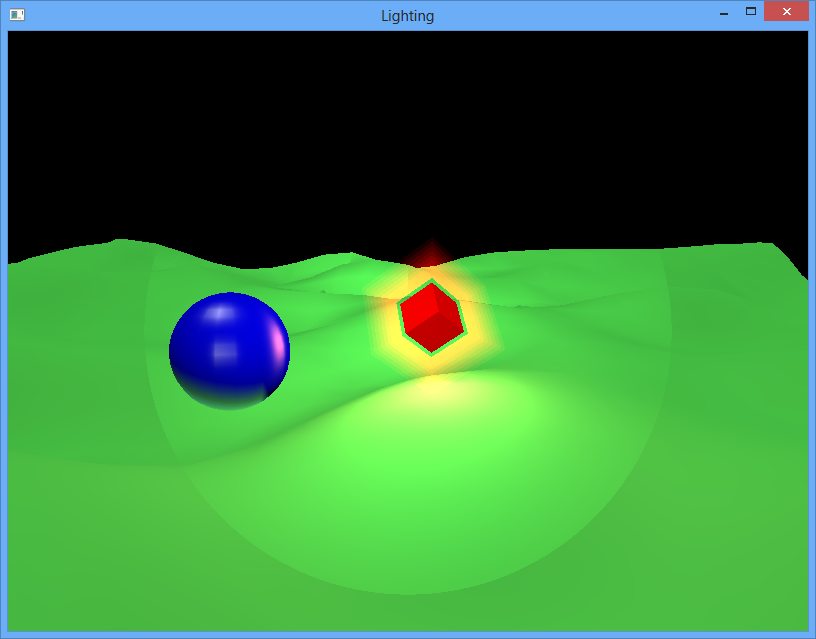
\includegraphics[width=1.0\textwidth]{lighting2.png}
\end{center}

\section{Fragment Shaders}
In general, a fragment shader is a very powerful concept, the application of which extends far beyond basic lighting computations. Fragment shaders are particularly well-suited for implementing hardware-accelerated raytracing techniques. You can get a good overview of what kinds of effects can be implemented in a single fragment shader by browsing the \emph{ShaderToy} website\footnote{\url{https://www.shadertoy.com/}}. Now, although understanding the techniques behind demos like \url{https://www.shadertoy.com/view/lsXGWl} in full detail is somewhat beyond the scope of our course\footnote{It is not too far beyond this course, though. Take a look here for a list of useful keywords, if you are interested: \url{http://www.iquilezles.org/www/articles/proceduralgfx/inspire2008.pdf}}, an easy starting point is trying to use a fragment shader to implement a simple Phong-lighted orthogonal projection of a sphere.

\begin{exercise}{4*}{1}
We shall be using the ``ShaderToy'' website in this exercise. Open the website and click ``New Shader''. You will be presented with the \texttt{main} function of an empty fragment shader. Recall that the shader must produce the value for the \verb#gl_FragColor# variable -- color of the pixel located at position \verb#gl_FragCoord#.

\begin{enumerate}
\item Suppose we are trying to render an orthogonal projection of a sphere. Our viewport is positioned so that the sphere is centered in the window and its height is exactly half the window's height. Let us start coding our shader by determining the pixels that belong to such a sphere.
\begin{lstlisting}
void main(void) {
    // Center and normalize coordinates
	vec2 uv = gl_FragCoord.xy - iResolution.xy*0.5;
	uv /= iResolution.yy*0.5;
	
	// Write red pixels for all points belonging to the sphere
	if (length(uv) < 0.5) {
		gl_FragColor = vec4(1, 0, 0, 1);
	}
	else {
		gl_FragColor = vec4(1, 1, 1, 1);
	}
}
\end{lstlisting}
\item Now for every pixel that does belong to the sphere you have to implement the following: 
\begin{enumerate}
\item Compute the position of the corresponding point on the sphere in 3D. Assume that sphere is centered at $(0, 0, 0)$ in camera coordinates.

Hint: Every point on the sphere satisfies $$x^2 + y^2 + z^2 = R^2.$$
\item Compute the normal at this point.
\item Assume the direction to the viewer is $(0, 0, 1)$ as usual.
\item Assume that the sphere is illuminated by a positional light source located at $(5, 2, 5)$. Compute the light direction and the reflection vectors.
\item Assume the sphere's diffuse color is red $(1, 0, 0)$, specular is white $(1, 1, 1)$, shininess is $15$, ambient light is $(0.1, 0.1, 0.1)$. Let the light source intensity be $(0.7, 0.7, 0.7)$ for both diffuse and specular components. Assume no attenuation. Given this information and the previously computed vectors, evaluate the Phong lighting model at the corresponding point on the sphere.
\item Apply gamma correction.
\item Apply HDR, if you find it necessary.
\item Finally, make the light position move around the sphere in a circle. I.e. do something like
\begin{lstlisting}
vec3 light_pos = vec3(5.0*cos(iGlobalTime), 2.0, 
				5.0*sin(iGlobalTime));
\end{lstlisting}
\end{enumerate}
\item As a result you will have implemented an animated rendering of a complete sphere done fully within a fragment shader (i.e. no ``standard graphics pipeline'' involved). The resulting image should look more or less as follows:
\begin{center}
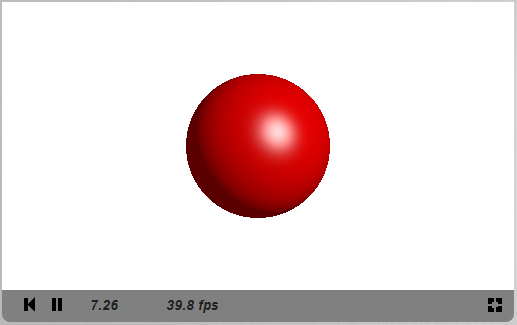
\includegraphics[width=0.7\textwidth]{sphere.png}
\end{center}
\item Submit the solution to this exercise in a text file \texttt{sphere.glsl} added to the archive. Note in the submission comment that you did solve this task.
\end{enumerate}
\end{exercise}

\end{document}
